\documentclass[12pt]{article}


\usepackage[a4paper,top=3cm,bottom=2.5cm,left=3cm,right=4cm,marginparwidth=1.75cm]{geometry}
\usepackage{tgtermes} % times font
\usepackage[T1]{fontenc}
\usepackage[german]{babel}
\linespread{1.25}
\usepackage{float}
\usepackage{hyperref}
\usepackage{graphicx}
\usepackage{datetime}
% IBID???
\usepackage[pagetracker,notes,backend=biber,doi=false,isbn=false,noibid,short]{biblatex-chicago}
%\usepackage{blindtext}
\usepackage{titlesec}
\usepackage{microtype}
\usepackage{bookmark}
\usepackage{xcolor}

\hypersetup{
    colorlinks,
    linkcolor={black!50!black},
    citecolor={blue!50!black},
    urlcolor={blue!60!black}
}
\emergencystretch 10pt

\title{Alkohol - Eine Gefahr für die Jugend in Baden-Württemberg?}
\bibliography{main}
\begin{document}
\pagenumbering{gobble}

\begin{titlepage}
    \begin{center}
        \vspace*{1cm}
 
        {\huge{Alkohol}}
 
        \vspace{0.7cm}
         {\Large Eine Gefahr für die Jugend in Baden-Württemberg?}
             
        \vspace{1cm}
 
        \textbf{Lukas Vogel \& Christian Krause}
              
             
        %\vspace{cm}
        \vfill
        %
\includegraphics[width=0.2\textwidth]{assets/gymox.png}
        \large
        Seminarkurs von Frau Titze 2023/2024\\
        Gymnasium Ochsenhausen\\
        Herrschaftsbrühl 12, 88416 Ochsenhausen\\
        \newdate{date}{13}{05}{2024}
        \displaydate{date}
             
    \end{center}
 \end{titlepage}

\clearpage
\tableofcontents
\clearpage
\pagenumbering{arabic}
\section{Einleitung}
Alkohol ist wichtiger Teil unserer Kultur. Auf vielen oberschwäbischen Festen, wie zum Beispeil Schützen, Öchslefest oder Fasching, wird Alkohol in großen Mengen konsumiert. Auch im Alltag wird von vielen oft Alkohol getrunken, zum Beispiel in Form von einem "Feierabendbier" oder ähnlichem. Vielen sind die tatsächlichen Gefahren von Alkohol aber nicht vollständig bewusst. Oft werden Risiken auch ignoriert oder verhamlost, was für Erwachsene, aber vor allem für Jugendliche eine große Gefahr ist. Daher werden wir uns in dieser Seminararbeit als Erstes mit den Gefahren von Alkohol beschäftigen. Anschließend werden wir den Alkoholkonsum von Jugendlichen in Baden-Württemberg anhand von Statistiken analyiseren. Anhand davon werden wir erörtern inwiefern dieser Konsum problematisch ist und welche möglichen Präventionsmaßnahmen es dagegen gibt.
\section{Gefahren \footnotesize{- Lukas}} % TODO Einleitung
% TODO die andere nescure quelle mit dem langen link
Der Alkohol bringt viele Gefahren mit sich – den meisten Konsumenten sind sie bewusst, aber sie werden dennoch ignoriert und der Alkohol wird in großen Mengen getrunken. 
Deswegen stellt sich die Frage: Sind die genauen Ausmaße von Alkoholkonsum doch nicht bekannt? 
Aus diesem Grund wollen wir uns in unserer Seminararbeit als Erstes mit den Risiken von Alkoholkonsum beschäftigen.%  in unserer Seminararbeit als Erstes über die Risiken von Alkoholkonsum aufklären.          
Alkohol ist ab dem ersten Tropfen schädlich für den Körper, denn der Alkohol wird über das Blut im Körper verteilt. Der Hauptbestandteil von Alkohol ist Ethanol, ein chemischer Stoff, der sowohl wasser- als auch fettlöslich ist. Für den Körper stellt dies die Gefahr dar, dass der Alkohol beziehungsweise das Ethanol durch seine Löslichkeit in jede Zelle eindringen und deshalb jeden Organismus beschädigen kann. Wichtig ist trotzdem zu wissen: Je mehr man an Alkohol trinkt, desto schädlicher ist es für den Körper \autocite{burger_bundes-gesundheitssurvey_2003}.\\
\subsection{Sucht}                                                                                                                
Zusätzlich kann das Trinken von Alkohol zu einer Sucht führen, bei der man abhängig von Alkohol wird. Es gibt verschiedene Anzeichen, um eine Alkoholsucht zu erkennen. Darunter fällt häufig auftretender Kontrollverlust beim Trinken, das ständige Denken an Alkohol, der anhaltende Konsum trotz ärztlich nachgewiesenen Folgeschäden und das Leugnen oder Verharmlosen des Alkoholkonsums \autocite{burger_bundes-gesundheitssurvey_2003}. \\
Unterschieden wird zwischen zwei Arten von Abhängigkeit. Zum einen wird man psychisch abhängig. Anzeichen einer psychischen Alkoholabhängigkeit sind ein starkes Verlangen nach Alkohol, der bereits erwähnte Kontrollverlust beim Trinken und Entzugserscheinungen bei Versuchen den Konsum zu reduzieren oder gar ganz aufzuhören. Anfänglich leidet der Konsument an inneren Unruhen, Stimmungsschwankungen und Konzentrationsstörungen. Allerdings gibt es auch Fälle, in denen es den Patienten schlechter geht. Schwere Entzugserscheinungen sind Störungen des Bewusstseins und Krampfanfälle sowie Panikattacken und Depressionen. In manchen Fällen kommt es sogar zu Halluzinationen. Die Nebenwirkungen des sogenannten Entzugssyndrom bewirken psychische Ängste und können je nach Menge des vorhergehenden Alkoholkonsums verstärkt werden und starke Schmerzen beim Patienten verursachen.\\
Zum anderen wird man physisch abhängig von Alkohol. Auch hier gibt es ähnliche Anzeichen einer Alkoholabhängigkeit, aber die physische Abhängigkeit hat andere Entzugserscheinungen. Anfänglich kommt es zu leichten Unruhen, sollte das neue Getränk mit Alkohol nicht in nächster Zeit erreichbar sein. Ist der Alkoholabhängige nur leicht betroffen hat es für ihn nur Auswirkungen wie beispielsweise Zittern, Schwindel oder Kreislaufprobleme. Sollte es eine Person schlimmer treffen, da sie normalerweise einen sehr hohen Alkoholkonsum hat, gehören Erbrechen, Schweißausbrüche und ein Schwächegefühl zu den Symptomen dazu. In extremen Fällen führt das Entzugssyndrom sogar zu Bluthochdruck und körperlichen Schmerzen. Im Zusammenhang mit anderen Vorerkrankungen führt das Entzugssyndrom in manchen Fällen auch zu Schlafstörungen oder Krampfanfällen. Die psychische und physische Alkoholabhängigkeit ist eng miteinander verbunden, da sie sich gegenseitig beeinflussen können \autocite{gohring_entzugserscheinungen_2022}. \\
Im Blick auf die beiden Abhängigkeiten und ihren Symptomen lässt sich erneut sagen, je mehr Alkohol man trinkt, umso schwerer ist es für den Körper, sich davon zu erholen und auch das Absetzen des Alkoholkonsum wird dadurch erheblich erschwert. \\
\subsection{Gesallschaftliche Folgen}                                                                                                                
Alkoholkonsum hat nicht nur Folgen am eigenen Körper, sondern kann sich auch auf die Gesellschaft und das Umfeld des Betroffenen auswirken. Übermäßiger Alkoholkonsum führt häufig zum Verlust von sozialen Verhaltensweisen, wodurch eine soziale Anbindung zu Freunde, Partner und letztendlich auch zur Familie verloren gehen kann. Es ist schwierig daraufhin ein eigenes Leben wieder aufbauen, denn auch auf die Arbeitswelt kann dies eine negative Auswirkung verursachen \autocite{burger_bundes-gesundheitssurvey_2003}. Wenn man auf der Suche nach Arbeit ist, wird es viele Bewerbungen brauchen, bis man einen Arbeitsgeber findet, der einen Bewerber einstellt, welcher zuvor ein Alkoholproblem hatte und sich von seinem sozialen Umfeld abgetrennt hat. Zusätzlich hätte er das Risiko, dass der Arbeitnehmer erneut in seine Alkoholsucht verfällt oder teilweise mit angestiegenem Alkoholpromillewert zur Arbeit erscheint. \\
Die Gefahr für das direkte Umfeld einer alkohol-trinkenden Person sind die damit verbundenen Unfälle im Verkehr, denn es kommt immer wieder vor, dass eine alkoholisierte Person am Straßenverkehr teilnimmt. Gefährdet wird dabei allerdings oft hauptsächlich die andere Person, die in den Unfall verwickelt ist. Fährt die Person mit hohem Promillewert mit einem Auto in einen anderen Menschen oder in ein Tier hinein, kommt meistens nur das Opfer zu Schaden. Im nüchternen Zustand ist man sich noch bewusst, dass man nicht mehr fahren wollte, wenn man später etwas getrunken hat, aber der Alkohol bringt die Gefahr mit sich, dass die Menschen dies dann oft nicht mehr selbst kontrollieren können und die Gefahren falsch einschätzen \autocite{burger_bundes-gesundheitssurvey_2003}. \\
Weiterhin führt ständiger Alkoholkonsum zu Gewaltbereitschaft und Kriminalität. Sie machen einen Großteil der Folgen von Alkoholkonsum aus. Damit verbunden schädigt man andere Menschen oder bekommt ein Problem mit dem Gesetz. Verbunden mit anderen Auswirkungen greift dies das psychische Denken der Personen an und in schlimmen Fällen für es nicht nur zu Depressionen, sondern auch zu Suizidgedanken \autocite{burger_bundes-gesundheitssurvey_2003}. \\
\subsection{Krebs}                                                                                                                
Eine weitere Gefahr verbirgt sich hinter dem Konsum von Alkohol und zusätzlichem Rauchen, denn in Verbindung mit anderen Rauschmitteln hat Alkohol eine deutlich verstärkte Wirkung auf den Körper und erhöht das Gesundheitsrisiko um ein Vielfaches. Der Grund dafür sind die krebserregenden Stoffe im Tabak, welche die Mundschleimhaut durchlässiger machen, sodass noch mehr Schadstoffe aufgenommen werden können \autocite{seufferlein_alkoholkonsum_2022}. \\
Dazu kommt, dass Krebs schon ohne zusätzlichen Einfluss ein großer Risikofaktor im Zusammenhang mit Alkoholkonsum ist. Laut der Weltgesundheitsorganisation ist Alkohol für sieben verschiedene Krebsarten verantwortlich und wird vom internationalen Krebsforschungszentrum in die höchste Risikogruppe mit unter anderem Asbest, Strahlung und auch Tabak eingestuft. Am häufigsten Treten dabei Darmkrebs und bei Frauen Brustkrebs auf. Nach der Managerin für Alkohol der Weltgesundheitsorganisation Doktor Feirreira-Borges sehen wir nicht die alkoholischen Schäden in unserer Region. In Europa sind über 200 Millionen Menschen bedroht, durch zu hohen Alkoholkonsum an Krebs zu erkranken. Dies ist im Vergleich zu anderen Kontinenten der Höchstwert. Zum einen kann es daran liegen, dass Viele nicht über das erhöhte Risiko einerKrebserkrankung Bescheid wissen \autocite{noauthor_beim_nodate}. Man kann jedoch auch davon ausgehen, dass viele Menschen dieses Risiko lediglich ignorieren, sich dessen vollen Umffang nicht Bewusst sind oder es einfach verharmlosen. \\
\subsection{Geschlechterspezifische Auswirkungen}
Bei Männern wurde durch eine Studie festgestellt, dass diejenigen, die über mehrere Jahre Alkohol konsumieren, bereits im mittleren Alter von 40 bis 60 Jahren Einschränkungen bei kognitiven Funktionen verursachen. Eintreffen können diese Folgen bei einem Konsum von im Schnitt mehr als 36 Gramm Alkohol pro Tag. Dies entspricht 370 Milliliter Wein oder 850 Milliliter Bier am Tag. Unterschiede bei den Einschränkungen im logischen Denken und anderen Gedächtnisfähigkeiten wurden zwischen Nichttrinkern und Menschen mit moderatem Alkoholkonsum  nicht festgestellt. Zudem wurden in der Studie bei Frauen ebenfalls keine Auswirkungen festgestellt, allerdings muss man bedenken, dass auch deutlich weniger Frauen an der Umfrage beteiligt wurden. Dennoch kann man aussagen, dass hoher Alkoholkonsum in frühem Alter schon Auswirkungen auf die Hirnaktivitäten im mittleren Alter hat \autocite{noauthor_alkohol_2014}. \\
Eine andere Gefahr betrifft dafür die Frauen. Alkoholkonsum während einer Schwangerschaft sollte unbedingt vermieden werden, denn dies birgt eine große Gefahr für das ungeborene Baby. Trinkt eine Frau während der Schwangerschaft Alkohol, so kann das Baby mit Alkoholschänden zur Welt kommen. Dabei reicht schon eine geringe Menge von 10 bis 60 Milliliter pro Woche, um den Embryo zu schädigen, denn der Alkohol ist länger im Kind vorhanden, da es noch nicht fähig ist, Alkohol so schnell abzubauen als ein erwachsener Mensch. Dadurch entstehen bei dem Baby größere Schänden. Häufig entstehende Schäden sind das Down-Syndrom oder ein offener Rücken. Damit schädigen die Mütter die Kinder nicht nur kurzzeitig, sie fügen ihrem eigenen Kind Schäden zu, welche sie ihr ganzen Leben lang beeinflussen können. Weltweite Studien ergeben, dass trotz dieser Gefahr ein Kind in 1000 Geburten mit Alkoholschäden auf die Welt kommt. Allerdings sollten schon die jugendlichen Mädchen mit Kinderwunsch im späteren Leben frühzeitig auf ihren Alkoholkonsum achten. Nach einer dänischen Studie von 1998 können bereits Mengen zwischen eins bis fünf Getränken in der Woche Folgeschäden für eine spätere Schwangerschaft verursachen und die Schwangerschaftsrate senken. Grundsätzlich wird jungen Frauen empfohlen vollständig auf den Alkoholkonsum zu verzichten, um einer Gefahr, die man selbst in der Hand hat, vorzubeugen \autocite[7-8]{butzer_alkohol_nodate}.\\ %Dass dadurch aber keine anderen Komplikationen entstehen, kann allerdings nicht garantiert werden. 
\subsection{Jugendliche}
Für Jugendliche speziell gibt es noch weitere Gefahren, welche Erwachsene weniger betreffen. Aus eigener Erfahrung können wir sagen, Buden beeinflussen den Alkoholkonsum von Jugendlichen besonders stark. Es ist ein sehr einfacher Weg für Jugendliche an Alkohol zu gelangen, um diesen konsumieren zu können. Dazu kommt, dass an Bude-Festen häufig auch Jugendliche dabei sind, die gerade einmal 14 Jahre alt sind und sie bekommen in Buden ebenfalls Alkohol. Dies führt dazu, dass junge Menschen schon sehr früh mit Alkohol in Kontakt kommen und dabei geht es nicht nur um Bier oder Sekt. In vielen Buden ist es für 14-jährige nicht schwer selbst an Schnaps zu kommen, denn dort kontrolliert sie niemand, sondern ihnen wird jedes beliebige Getränk ausgeschenkt. Zusätzlich kommt es auf Festen des Öfteren dazu, dass sich Jugendliche in der Gruppe gezwungen fühlen auch etwas zu trinken, obwohl sie es eigentlich garnicht wollen. Sätze wie "ach komm, ein Bier geht schon, das macht doch nichts“ oder "jetzt sei doch kein Looser, trink was mit uns“ sind keine Seltenheit mehr. Speziell die jungen Personen trauen sich in solchen Situationen nicht "nein“ zu sagen und unterliegen dann dem Gruppenzwang. Diese Vorfälle betreffen nicht nur Buden, hinzu kommen Dorffeste, Feste von Fußball- oder Musikvereinen und private Partys zu Hause. Viele Jugendliche kommen dadurch immer wieder sehr früh sehr einfach an Alkohol und von den Gefahren wissen nur selten etwas, denn häufig wird Alkohol unter Jugendlichen als "cool“ empfunden und so dargestellt. Wer also keine Alkohol trinkt, riskiert aus einer Gruppe ausgeschlossen zu werden. Gruppenzwang ist also große Gefahr, die den Alkoholkonsum von Jugendlichen deutlich erhöht.\\
Um auf die privaten Hauspartys zurück zu kommen, sie sind eine weitere Gefahr für Jugendliche, da sie wieder eine einfache Möglichkeit sind an Alkohol zu kommen. Dafür braucht es nur ein paar Eltern, die ihren Kinder schon früh Alkoholkonsum erlauben und dies führt zum nächsten Gefahrenfaktor, die Eltern. Die Eltern nehmen einen besonderen Einfluss auf die Jugendlichen als Vorbild für Alkoholkonsum. Die Jungen nehmen sich ein Beispiel vom Alkoholkonsum des Vaters, während Mädchen von beiden Elternteilen beeinflusst werden. Auch die Aufmerksamkeit, die die Jugendlichen von ihren Eltern bekommen kann ein entscheidender Faktor sein. Passen diese nicht auf ihre Kinder auf, führt dies häufig zu erhöhtem Alkoholkonsum. Eltern können ihren Kindern Regeln zum Alkoholkonsum vorschreiben, um einen positiven Einfluss zu verursachen, aber sie können eben auch einen negativen Einfluss haben. Dies macht Eltern mit risikoreichem Alkoholkonsum zu einer Gefahr für ihre eigenen Kinder \autocite[27]{kuhn_empfehlungen_nodate}. \\
\subsection{Fazit}
Zusammenfassend lässt sich sagen, egal ob Krebsrisiko, Hirnschädigungen oder Alkoholgeburten, Alkoholkonsum bringt viele Gefahren mit sich und dabei reicht auch manchmal schon ein moderater Alkoholkonsum. Dennoch gilt, je mehr Alkohol man konsumiert, umso schädlicher wird es für den Körper. Auch bringt man nicht nur sich selbst in Gefahr. Unter hohem Alkoholkonsum kann man die Kontrolle über seinen Körper nicht mehr garantieren und dabei auch andere in seinem Umfeld gefährden. Die Eltern selbst, die eigentlich eine Schutzfunktion für die Kinder und Jugendlichen darstellen sollten, können auch eine Gefahr für übermäßigen Alkoholkonsum ihrer Kinder sein, denn sie gelten für viele als Vorbild und haben dadurch einen großen Einfluss. 


\section{Alkoholkonsum in Baden Württemberg \footnotesize{- Christian}}
\subsection{Vergleich zu anderen Bundesländern}
Viele haben das Vorurteil, dass zwischen dem Trinkverhalten in den nördlichen und den südlichen Bundesländern in Deutschland ein großes Gefälle besteht und in Süddeutschland deutlich mehr Alkohol als in Norddeutschland konsumiert wird. Ein Beispiel dafür ist das bayrische Oktoberfest, bei dem enorme Mengen an Alkohol konsumiert werden. Es wird auch als das größte Drogenfestival in Deutschland bezeichnet \autocite{effern_munchen_2023}. Auch in Baden-Württemberg und in unserer direkten Umgebung gibt es viele Feste und Bräuche, bei denen traditionell viel Alkohol getrunken wird, zum Beispiel Schützen oder Fasching. Die Wissenschaft ist sich allerdings uneinig ob dieses Vorurteil wirklich zutrifft. Es gibt Studien die behaupten, dass es durchaus ein Gefälle zwischen dem Trinkverhalten im Norden und im Süden Deutschlands gibt \autocite{meyer_regionale_1998}. Eine andere Studie behauptet wiederum, dass diese Differenzen nur durch falsche Datenerhebung hervorgerufen werden \autocite[781]{kraus_einfluss_2001}. Um diese Behauptungen genauer zu analysieren haben wir die Methoden dieser Studien untersucht: \\
Die Nord- und Südcluster wurden anhand von vergleichbaren Konsummustern definiert. In den südlichen Bundesländern wird mehr Bier getrunken, während im Norden mehr Wein und Spirituosen getrunken werden. Zum Südcluster gehören Nordrhein-Westfalen, Hessen, Rheinland-Pfalz, Saarland, Baden-Württemberg und Bayern und der Nordcluster besteht aus Niedersachsen, Hamburg, Schleswig-Holstein, Mecklenburg-Vorpommern, Brandenburg, Berlin, Sachsen, Sachsen-Anhalt und Thüringen. Bremen würde vom Konsummuster eher in den Südcluster passen und stellt daher eine Ausnahme dar. Trotz dieser unterschiedlichen Konsummuster können bei der konsumierten Menge an Reinalkohol und bei der Prävalenz von riskantem Konsum keine signifikanten Unterschiede zwischen den Nördlichen und den Südlichen Bundesländern festgestellt werden \autocite[780]{kraus_einfluss_2001}.\\
Dieses Ergebnis wurde mit einer Analyse der Bundesstudien zum Konsum psychotischer Substanzen 1995 und 1997 erzielt \autocite[777]{kraus_einfluss_2001}. Die von Meyer et al. \autocite{meyer_regionale_1998} vorgenommene Sekundäranalyse der Gesundheitssurvey Ost-West kommt allerdings zu dem Ergebnis, dass es signifikante Unterschiede in der Konsumierten Menge an Reinalkohol und der Prävalenz von Riskantem Konsum zwischen Nord- und Süddeutschland gibt. Diese Ergebnisse wurden aber vermutlich dadurch stark verfälscht, dass die Angabe der Alkoholmenge pro Tag als Alkoholmenge pro Trinktag interpretiert wurde \autocite[781]{kraus_einfluss_2001}. Daher sind die Ergebnisse dieser Studie vermutlich nicht aussagekräftig und wir können davon ausgehen, dass es zwischen Nord- und Süddeutschland keine signifikanten Unterschiede in Trinkmenge und Prävalenz für riskanten Alkoholkonsum gibt.\\
Wenn man allerdings die einzelnen Bundesländer genauer betrachtet fällt auf, dass in Bayern tatsächlich überdurchschnittlich viel Alkohol konsumiert wird \autocite[778]{kraus_einfluss_2001}. In Baden Württemberg wird allerdings durchschnittlich relativ wenig Alkohol pro Tag getrunken. Auch der riskante Alkoholkonsum ist relativ gering. Da wir uns in unserer Seminararbeit hauptsächlich auf den Alkoholkonsum von Jugendlichen fokussieren wollen wäre eine solche Statistik zum durchschnittlichen Alkoholkonsum von Jugendlichen in den verschiedenen Bundesländern natürlich interessant. Bei unserer Recherche haben wir eine solche spezifische Statistik allerdings nicht gefunden.\\
\subsection{Analyse der Krankenhausstatistik}

Um aber trotzdem eine Aussage über den Alkoholkonsum von Jugendlichen in Deutschland zu treffen, haben wir die Daten auf der Plattform GENESIS (Gemeinsames Neues Statistisches Informations-System) \autocite{noauthor_statistisches_nodate} verwendet. Auf GENESIS findet sich ein breit gefächertes Datenangebot von den statistischen Landesämotern und dem Statistischen Bundesamt. Dieses enthält u.a. einen Datensatz mit dem Bundesland, Alter, Geschlecht und der Hauptdiagnose aller Krankenhauspatienten in Deutschland \autocite{noauthor_genesis_nodate}. Aus dieser Statistik haben wir alle Krankenhausaufenthalte von Jugendlichen bis 19 Jahren, die aufgrund von einer Alkoholintoxikation (Diagnose ICD-10 F10.0 \autocite{noauthor_icd-10-code_nodate}) im Krankenhaus waren extrahiert. In der folgenden Grafik sieht man diese im Durchschnitt pro 100.000 Einwohner des jeweiligen Bundeslandes über die letzten 15 Jahre aufgelistet.

\begin{figure}[H]
    \centering
    \includegraphics[scale=.7]{"assets/Alkohol_Bundesländer_avg_15_Jahre.png"}
    \caption{Alkoholbedingte Krankenhausaufenthalte von Jugendlichen in Abhängigkeit des Bundeslandes}
    \label{fig:Krankenhausaufenthalte_1}
\end{figure}

Für die Bevölkerungsanzahlen zur Normalisierung der Statistik wurde die Bevölkerung des jeweiligen Bundeslandes zum jeweiligen Zeitpunkt verwendet \autocite{noauthor_statistisches_2024}. Die Werte wurden mit Python berechnet und die Grafik wurde mit der Python Bibliothek Matplotlib \autocite{noauthor_matplotlib_nodate} erstellt. 

Es fällt auf, dass die Werte für kleine Bundesländer (Saarland, Hamburg und Berlin) stark abweichen. Das könnte an den geringen Fallzahlen liegen, die dann zu Extremwerten führen. Die absoluten Fallzahlen schwanken zum Beispiel im Saarland über die Jahre von 200 bis knapp 400. Ein weiterer wichtiger Aspekt, der bei der Analyse dieser Daten beachtet werden muss, ist der Länderaustausch von Patienten. Das Bundesland, in dem ein Patient behandelt wird, muss nicht mit dem Wohnort des Patienten übereinstimmen. Das kann aufgrund der Normalisierung der Daten zu einer Verfälschung der Ergebnisse führen. Auf GENESIS ist auch eine Statistik verfügbar, die statt dem Ort des Krankenhauses den Wohnort der Patienten angibt \autocite{noauthor_genesis_nodate-1}.

\begin{figure}[H]
    \centering
    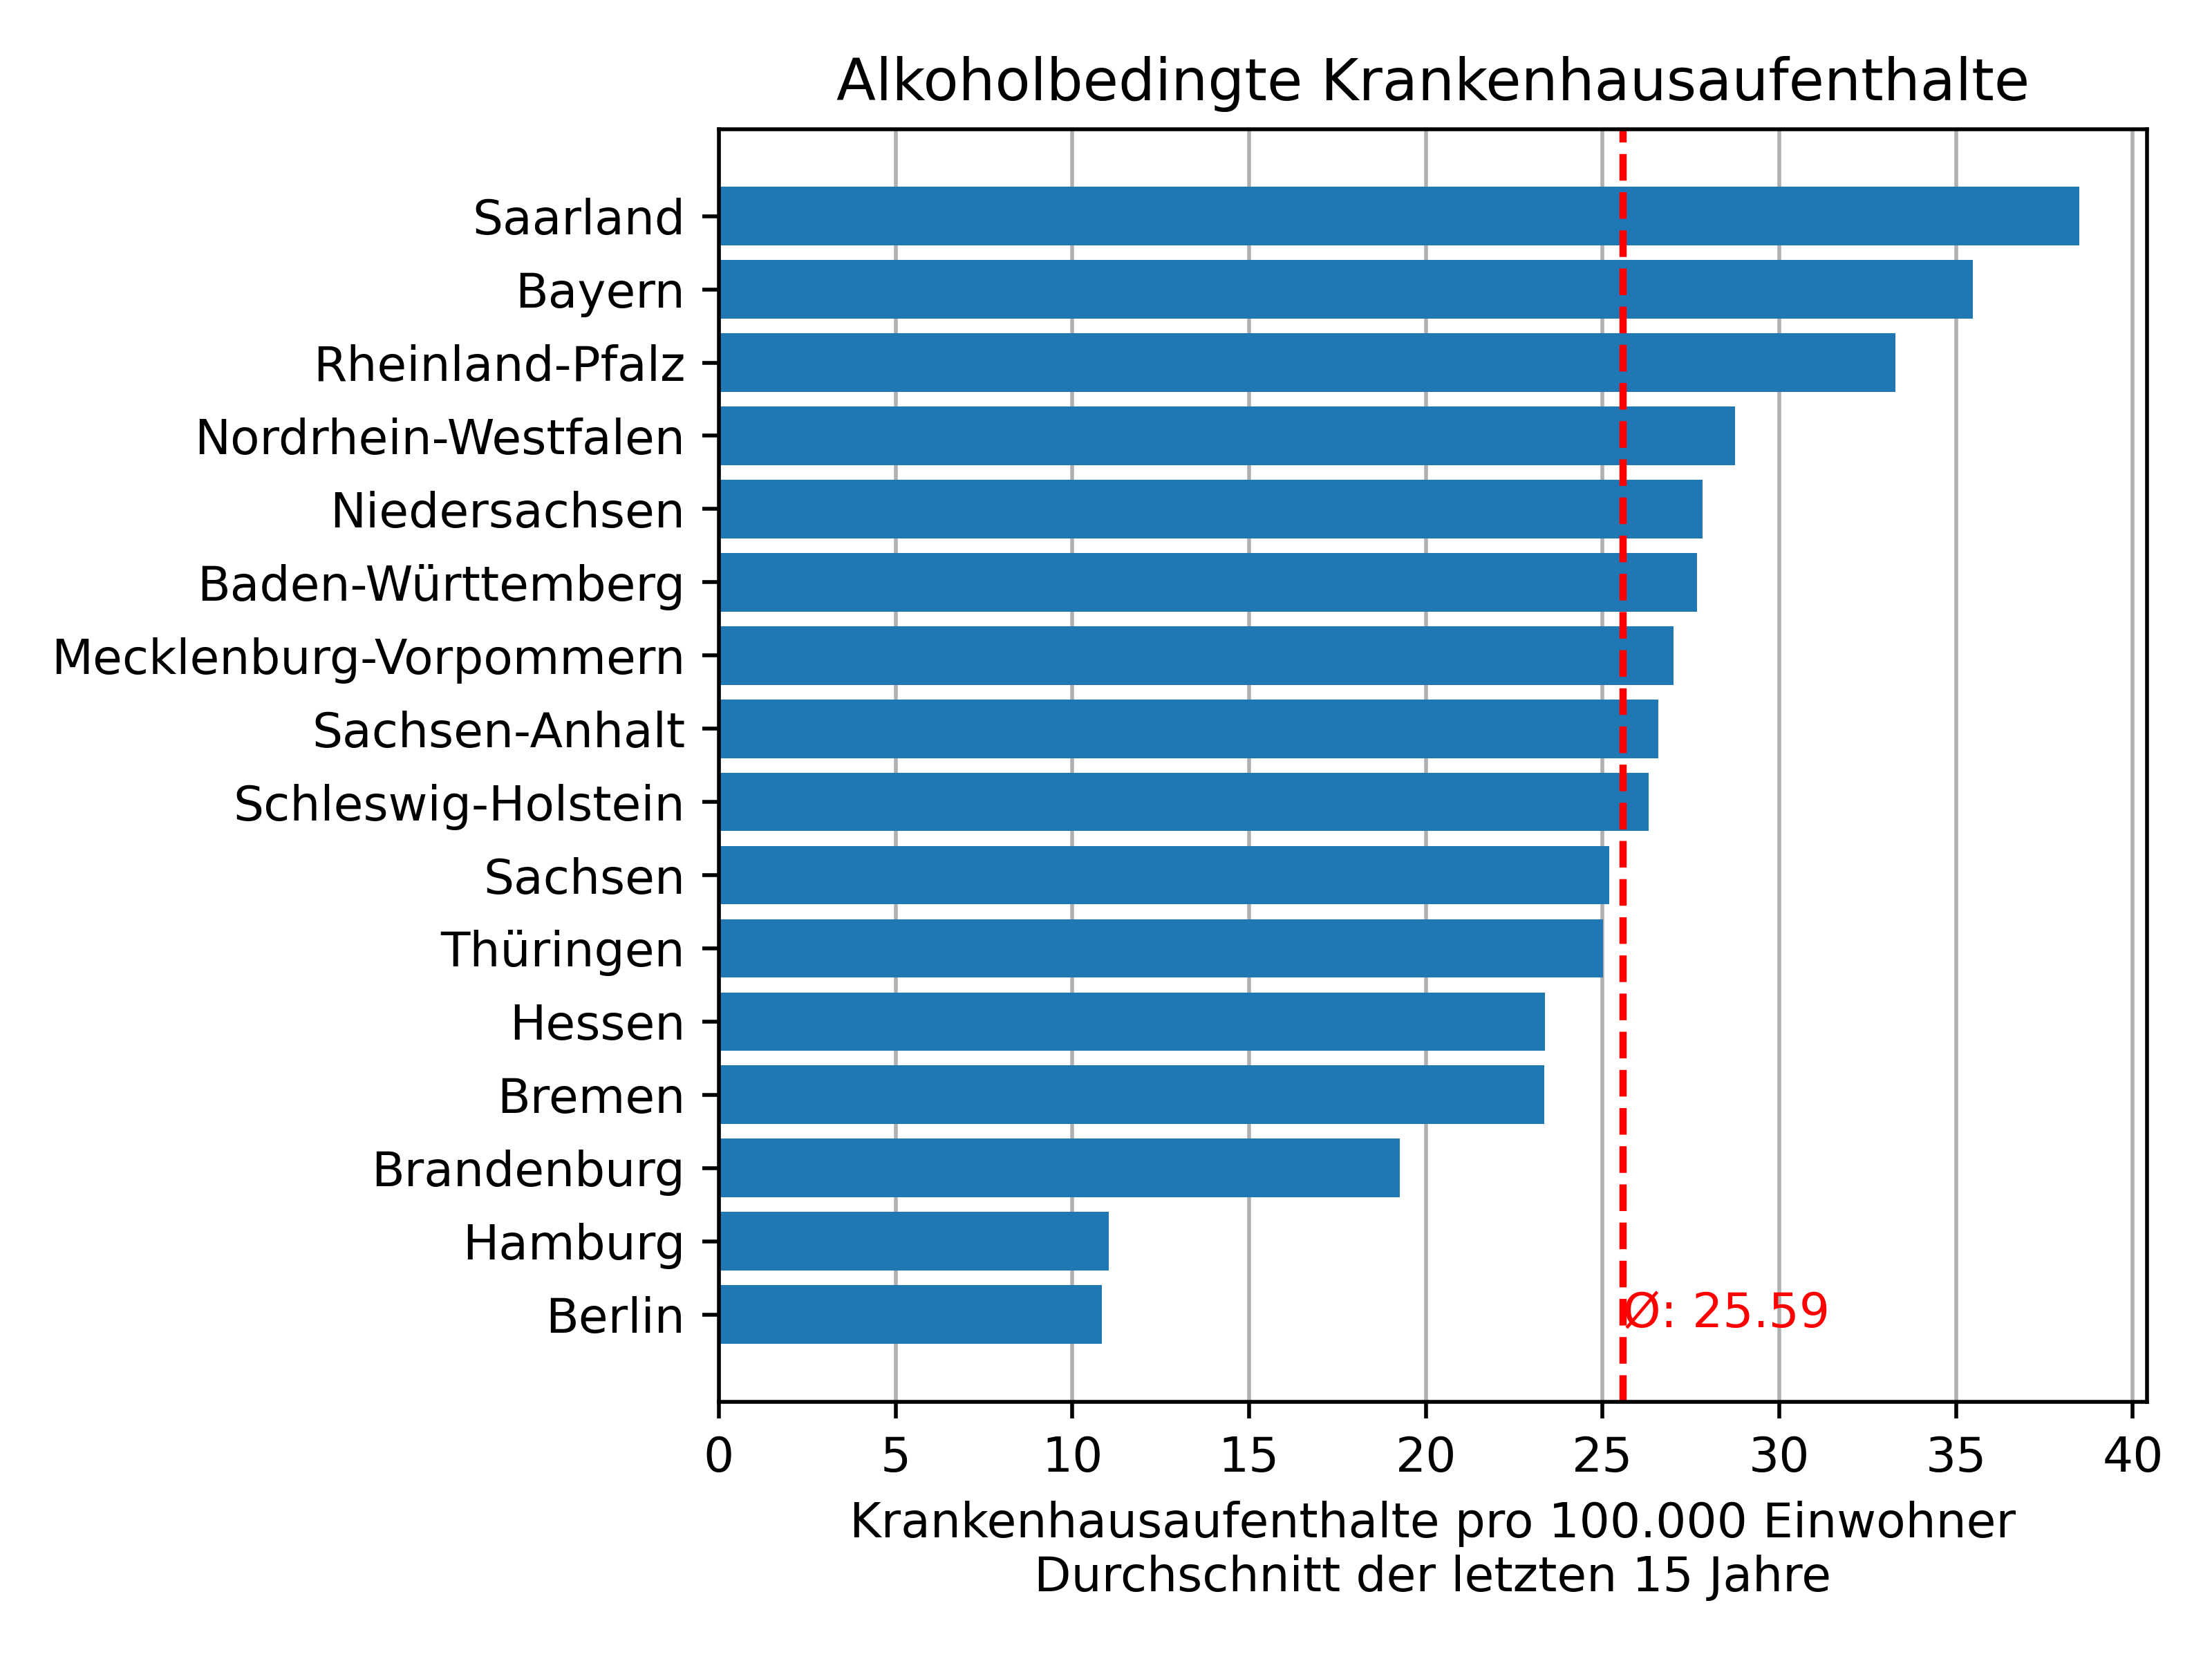
\includegraphics[scale=.7]{"assets/Alkohol_Wohnort_avg_15_Jahre.png"}
    \caption{Alkoholbedingte Krankenhausaufenthalte von Jugendlichen in Abhängigkeit des Wohnortes}
    \label{fig:Krankenhausaufenthalte_2}
\end{figure}

Grafik \ref{fig:Krankenhausaufenthalte_2} wurde mit den gleichen Methoden wie Grafik \ref{fig:Krankenhausaufenthalte_1} erstellt. Patienten deren Wohnort unbekannt ist und Patienten, die aus dem Ausland kommen wurden in dieser Grafik ignoriert. 
Die Werte für die meisten größeren Bundesländer sind nahezu gleich geblieben, da dort der Anteil der Patienten, die in einem anderen Bundesland behandelt wurden im Vergleich zu den Patienten, die in ihrem Heimatbundesland behandelt wurden sehr klein ist. Die Werte der kleineren Bundesländer (Hamburg, Berli<n, Bremen und Saarland) sind dagegen stärker gesunken, vor allem bei Bremen. Das könnte daran liegen, dass ein Teil der Patienten, die zum Beispiel in einem Krankenhaus in Bremen behandelt wurden aus dem umliegenden Niedersachsen kommen. Dass die hohen Werte im Saarland kein Fehler in der Statistik sind, sondern ein reales Problem darstellen zeigt sich auch in diesem Artikel \autocite{noauthor_saarland_nodate}, der das Problem des Alkoholmissbrauchs von Jugendlichen im Saarland beschreibt. 
\\
Grafik \ref{fig:Krankenhausaufenthalte_1} und Grafik \ref{fig:Krankenhausaufenthalte_2} stellen den Durchschnitt der alkoholbedingten Krankenhausaufenthalte von Jugendlichen über die letzten 15 Jahre dar. Die folgende Grafik beschäftigt sich dagegen mit dem Zeitlichen Verlauf der alkoholbedingten Krankenhausaufenthalte von Jugendlichen in Baden-Württemberg und in Deutschland von 2000 bis 2022.
\begin{figure}[H]
    \centering
    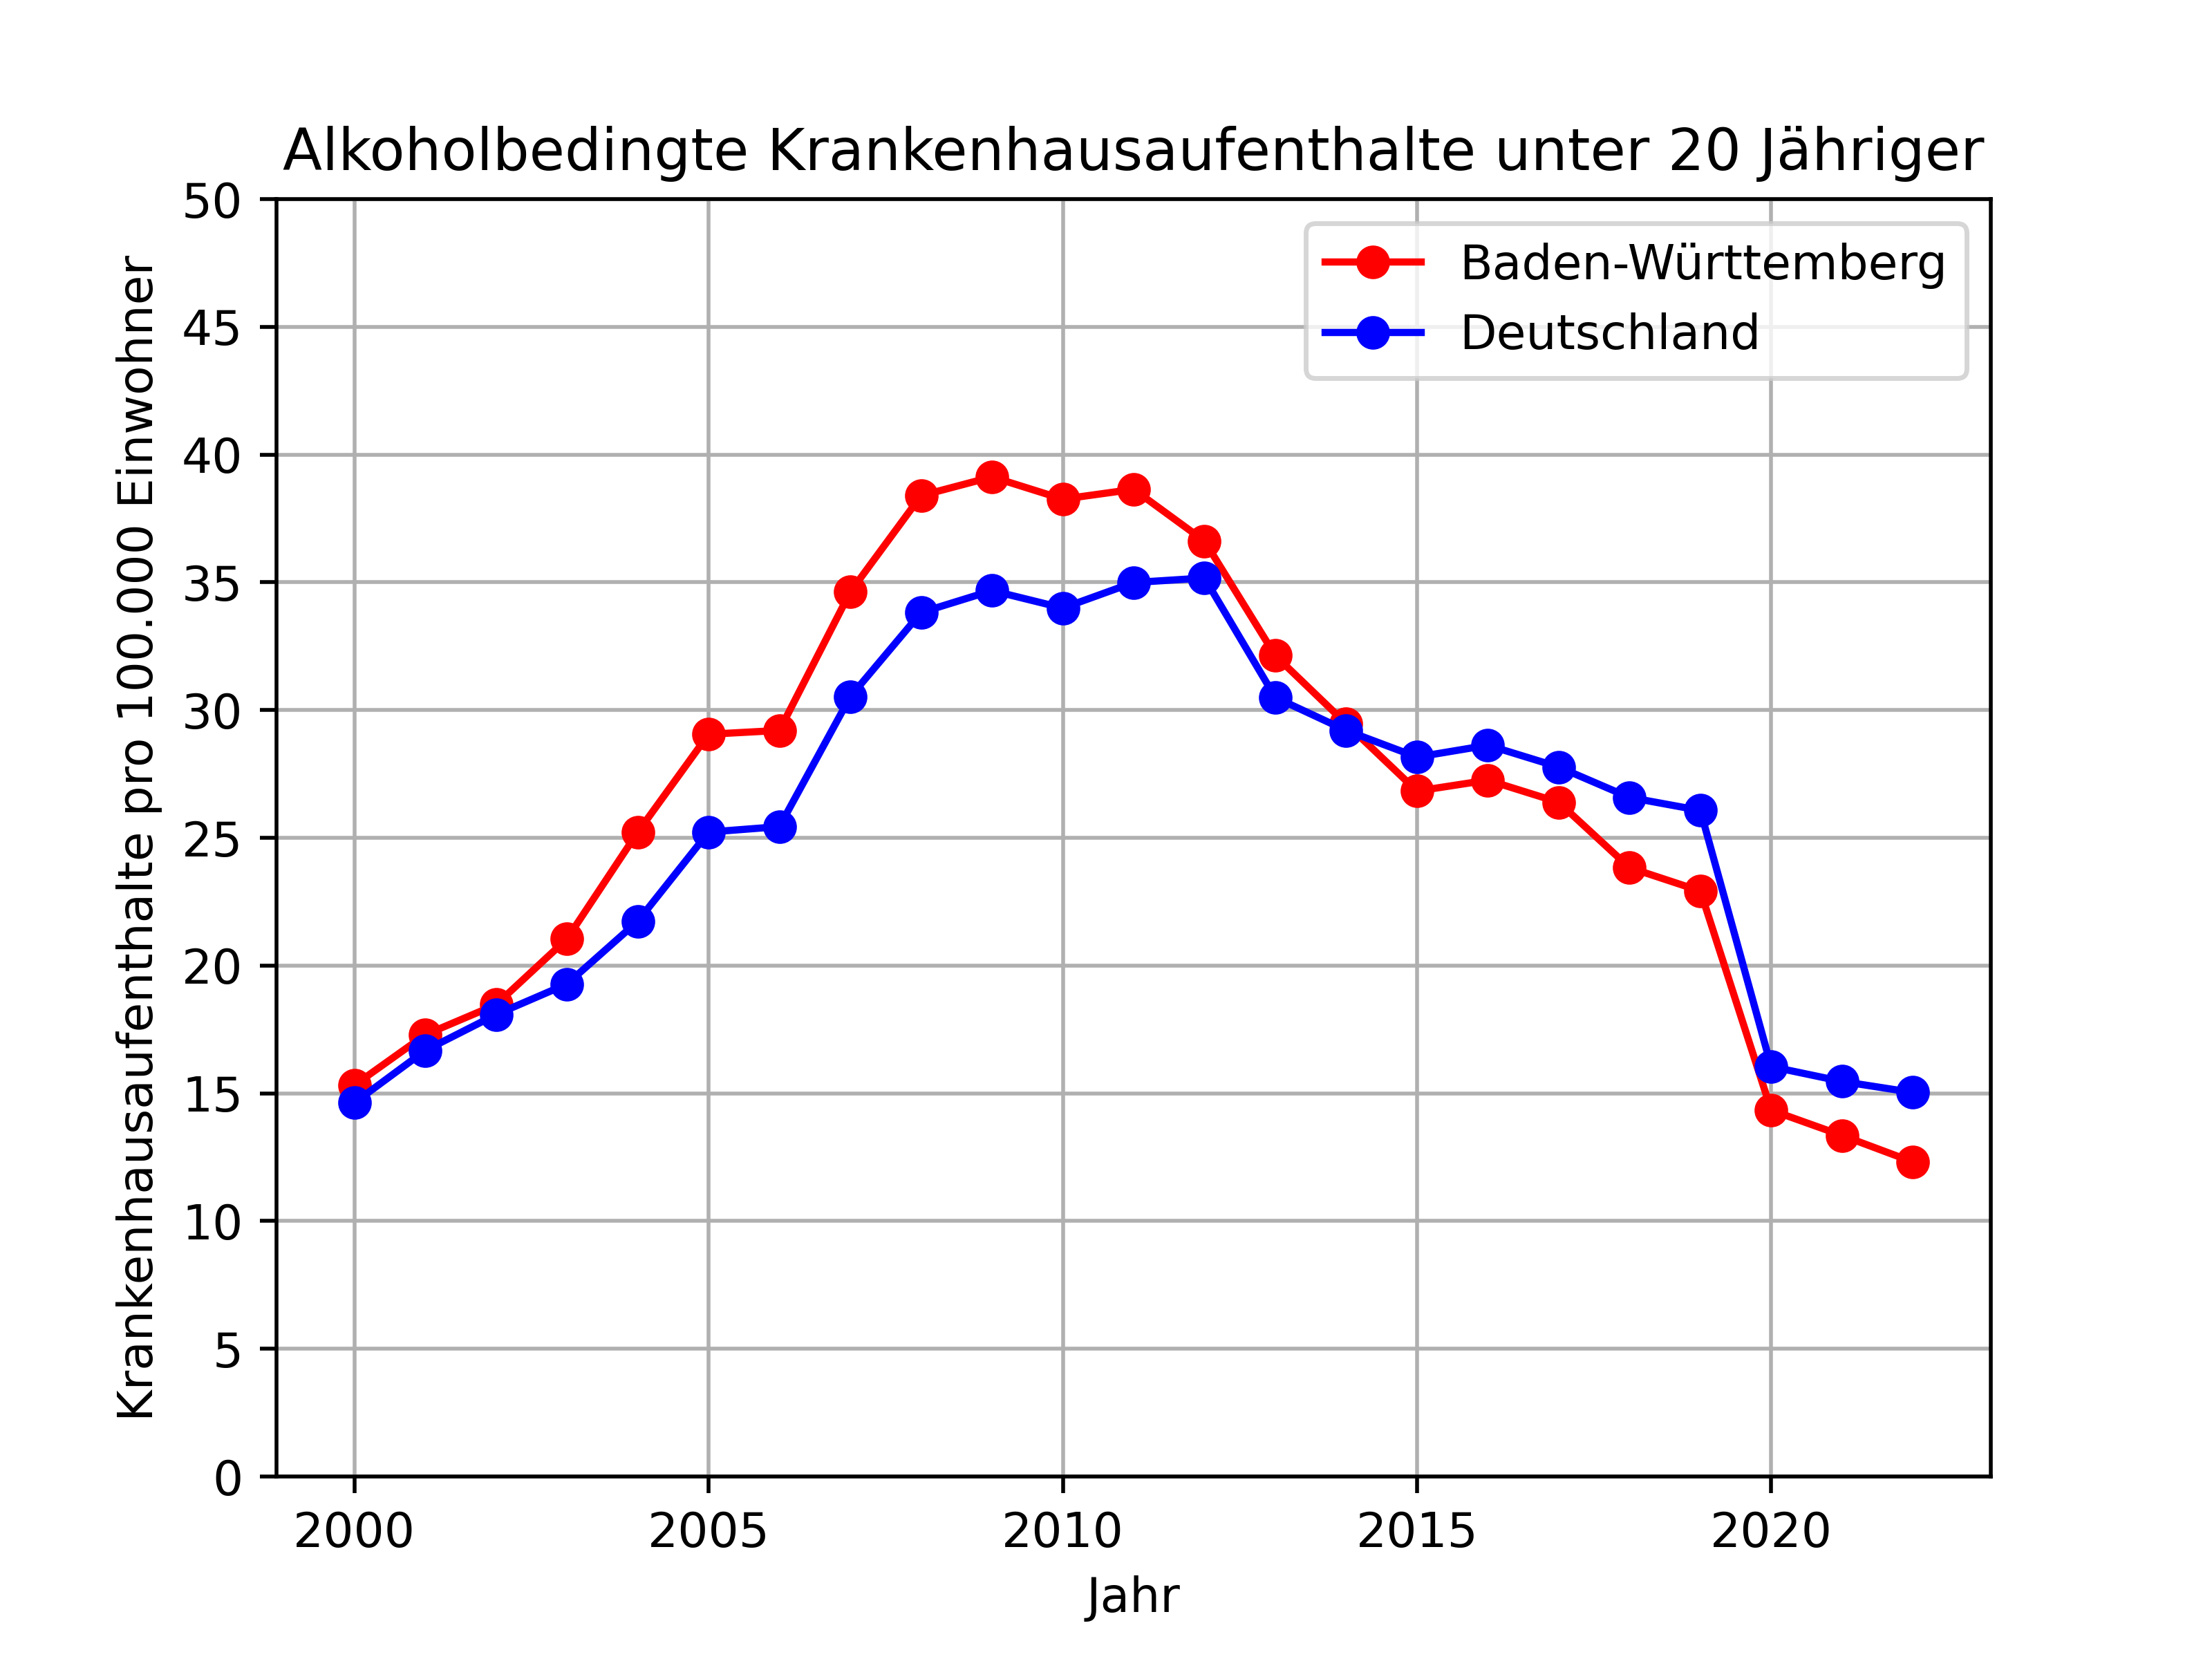
\includegraphics[scale=.7]{"assets/Alkohol_BW_Ges.png"}
    \caption{Alkoholbedingte Krankenhausaufenthalte von Jugendlichen von 2000 bis 2022}
    \label{fig:Krankenhausaufenthalte_3}
\end{figure}
Diese Grafik wurde ebenfalls mit den oben genannten Methoden erstellt.
Man sieht, dass sich die Verläufe von Baden-Baden Württemberg und Deutschland stark ähneln. Sie erreichen bis 2010 Höchstwerte und fallen bis 2019 auf ein Niveau von ca. 25 Krankenhausaufenthalte pro 100.000 Einwohner ab. Auch der Einfluss der Corona-Pandemie auf diesen Verlauf ist sehr gut zu erkennen, die Werte aus den Jahren 2020, 2021 und 2022 sind deutlich geringer als die der Jahre davor. Sogar die Tagesschau berichtet von derartigen Effekten \autocite{tagesschaude_weniger_nodate}.

Insgesamt kann man sagen, dass man auch an der Krankenhausstatistik sieht, dass der riskante Alkoholkonsum bei Jugendlichen in Baden-Württemberg von Jugendlichen nur geringfügig höher als der Bundesdurchschnitt ist.

\section{Eigene Umfrage \footnotesize{- Lukas}}
Neben den vorherigen allgemeinen Auswertungen fanden wir es auch interessant, uns ein Bild von unserem eigenen Umfeld zu machen. Dafür haben wir über eine Iserv Umfrage über den Zeitraum von einer Woche alle Schüler der Klasse 10 sowie der Jahrgangsstufen 1 und 2 bzu ihrem Alkoholkonsum befragt.
\subsection{Auswertung}
Insgesamt haben 101 der 129 Schüler an der Umfrage teilgenommen, was einer Beteiligung von ungefähr 78 Prozent entspricht.
31 Stimmen sind von der Jahrgangsstufe 2, die somit rund 30 Prozent aller Beteiligten ausmachen. Am meisten teilgenommen haben die Schüler der Jahrgangsstufe 1. Hier haben sich 40 Schüler (39,6\%) die Zeit genommen, um die Fragen zu beantworten. Rein von der Anzahl der Teilnehmer nahmen am wenigsten Schüler der Klasse 10 teil. Von Ihnen haben 30 Schüler an der Umfrage teilgenommen. 
Jedoch muss man berücksichtigen, dass in der Klassenstufe 10 deutlich weniger Schüler sind als in den anderen Stufen. Somit ist der prozentuale Anteil der teilnehmenden Schüler in Klasse 10 mit 77\% wiederum am zweithöchsten nach der Jahrgangsstufe 1 (83\% aller Schüler in dieser Stufe). Die Jahrgangsstufe 2 hatte sich mit 73\% dennoch ebenfalls sehr gut an der Umfrage beteiligt.\\
Für uns sehr passend ist die ausgeglichene Beteiligung von männlichen und weiblichen Schülerinnen und Schüler, da es uns ermöglicht, die Resultate auf beide Geschlechter zu beziehen. 50 Schüler stehen in der Umfrage 49 Schülerinnen gegenüber, während lediglich 2 keine Angabe zu ihrem Geschlecht geben wollten. 
Vor dem Absenden der Umfrage haben wir uns vorgestellt, dass die meisten zwischen 14 und 15 das erste Mal Alkohol getrunken haben und diese Vermutung wurde letztendlich auch bestätigt. Über die Hälfte haben in diesem Zeitraum ihren ersten Kontakt zu Alkohol gehabt, wobei relativ viele Schüler auch mit 13 schon das erste mal Alkohol getrunken haben. Nur selten wurde in jüngerem oder älterem Alter das erste Mal getrunken. Interessant war auch, dass 14 Leute noch nie Alkohol getrunken haben. \\
Bei der Frage, wie oft die Abgefragten aktuell noch trinken ist das Ergebnis ziemlich ausgeglichen. Zwischen "seltener als einmal im Monat“ und "häufiger als einmal in der Woche“ gibt es abgesehen von "mehrmals im Monat“ (24\%) kaum prozentuale Unterschiede (zwischen 11\% - 15\%). Von den ursprünglich 14 Schülern, welche noch nie Alkohol getrunken haben, trinken zwischenzeitlich neun weitere keinen Alkohol mehr. Das bringt uns zu dem Schluss, dass manche einmal probiert und danach aber nichts mehr getrunken haben, wobei aber sicherlich auch Schüler dabei sind, die einfach so aufgehört haben. Dafür kann es verschiedene Anlässe geben, beispielsweise aus körperlichen oder gesundheitlichen Gründen, wie zum Beispiel einer entstandenen Allergie.\\ 
Etwas überraschend fanden wir, dass Mischgetränke und purer Schnaps mit Abstand am beliebtesten waren. Knapp 70 Prozent der Befragten trinken sehr gerne Mischgetränke, wenn sie auf einer Party sind und mit 39 Prozent trinken die Befragten am zweitmeisten Schnaps (Shots), was doch ein deutlicher Abstand zu Bier, welches an dritter Stelle steht (32\%). Etwas irritierend fanden wir allerdings, dass bei dieser Frage nur noch 22 Leute mit "keinen Alkohol“ abgestimmt haben. Wir konnten es uns nur so erklären, dass diese eine Person abgestimmt hat, welches Getränk sie früher am liebsten getrunken hat. Natürlich kann man einzelne Schüler, die zufällig oder unwahr abgestimmt haben, nicht ausschließen. \\
Unsere siebte Frage lautete "Wie viel trinkst du normalerweise an einem Tag?“. Interessiert hat uns dabei zu erfahren, wie viel die Jugendlichen in unserem Alter an Getränken an einem Abend trinken. Wie bereits erwartet trinken die meisten zwischen drei und vier Getränke pro Party (23.76\%). Etwas darunter liegt die Auswahl zwischen fünf bis sechs (15.8\%) und ein bis zwei Getränken (10.9\%). Nur sehr selten trinken die Schüler mehr als sieben oder acht Getränke, wobei es natürlich ein paar Ausreißer gibt, die sogar mehr als 10 Getränke über den ganzen Abend trinken. Sehr verwunderlich ist allerdings, dass 37 Befragte angeben, sie trinken den ganzen Abend über nichts. Damit ist die Zahl der vorherigen Personen, die keinen Alkohol trinken innerhalb der letzten zwei Fragen um 14 Personen gestiegen. Das ist eine sehr große Anzahl, um von einem versehentlichen falschen abstimmen ausgehen zu können. Eine Möglichkeit für diese Ausreißer könnte die ungenaue Fragestellung sein, man könnte die Frage auch so interpretieren, dass nicht nur Trinktage, sondern alle Tage gemeint ist.\\
Natürlich war es für uns auch interessant zu sehen, zu welchem Anlass gerne getrunken wird, hierbei war eine Mehrfachauswahl möglich. Jede befragte Person, abgesehen von denen, die keinen Alkohol trinken, hat angeben, dass sie auf Partys und Geburtstagen Alkohol konsumieren. Weiter verbreitet ist der Konsum an Festen von Vereinen oder an Fasching. Die Hälfte der Alkohol konsumierenden Schüler trinken auch, wenn sie bei der Verwandtschaft sind. Nur selten wird Alkohol allein oder am Feierabend getrunken (5-7\%). Auch die achte Frage ergibt erneut eine neue Anzahl an nicht Alkohol trinkenden Personen. 21 Schüler haben "Kein Alkohol“ angegeben. Zwar liegt der Wert wieder sehr eng bei den ersten Angaben, allerdings bringt dieser Wert ein anderes irritierendes Ergebnis mit sich. Mit einem Blick auf die Schüler, die angegeben haben, auf Partys und Geburtstagen Alkohol zu konsumieren (81 Schüler) und dann mit Blick auf diejenigen, die keinen Alkohol trinken (21) bemerkt man, dass insgesamt 102 Schüler abstimmen hätten müssen. Das Problem dabei ist, dass aber nur 101 Schüler an der Umfrage teilgenommen haben und es somit zu einer Überschneidung gekommen sein musste. Das ist vermutlich wieder auf einzelne Schüler zurückzuführen, die zufällig oder unwahr abgestimmt haben.\\ 
Im Hinblick auf Alkoholkonsum ist es immer wichtig zu schauen, trinkt man aus eigenem Antrieb oder wird man mehr dazu gedrängt, sei es Gruppenzwang, den man hat oder andere Menschen um einen herum, die versuchen dich dazu zu bringen, Alkohol zu trinken. Diese Frage haben wir uns auch gestellt und ebenfalls in unsere Umfrage mit aufgenommen. Erfreulich für uns war, dass 33 Schüler angaben, sie trinken immer aus eigenem Antrieb und 31 weitere, die immerhin meistens aus eigenem Antrieb trinken. Lediglich sieben Schüler werden manchmal zum Alkoholkonsum gedrängt und leider auch drei, die fast immer dazu gedrängt werden. Acht Schüler waren so ehrlich und haben angegeben, sie trinken immer aus eigenem Anlass, aber drängen andere auch dazu, etwas zu trinken. Auch hier variiert die Zahl der nicht Alkohol trinkenden Personen wieder und es sind nur noch 19.
Oft gibt es auch mal einen bestimmten Grund, wieso man an einem Tag keinen Alkohol trinken möchte. Bei unserer Umfrage haben die Teilnehmer bei Frage zehn als häufigsten Grund "keine Lust“ angegeben (64.4\%). Auch hier war wieder eine Mehrfachauswahl möglich. Andere Gründe, die viele angegeben haben, waren ein wichtiger Termin, beispielsweise ein Fußballspiel oder eine Klassenarbeit, am nächsten Tag (48.5\%) oder die Teilnahme am Straßenverkehr (43.6\%). Ebenfalls ungefähr gleich angegeben war der Grund, die anderen trinken auch nicht und es hat gesundheitliche Folgen (27-31\%). Die Anzahl der nicht Alkohol konsumierenden Schüler ist wieder auf 22 Schüler angestiegen, wobei dieser Wert bei dieser Frage etwas ungenau sein könnte, da zum Beispiel eine Person angegeben haben könnte, sie trinkt nicht aus gesundheitlichen Gründen und dann nicht mehr weitergelesen hat. \\
Jetzt hat sich nur noch die Frage gestellt, wie schätzen die Befragten ihren Konsum überhaupt selbst ein? Die meisten gehen davon aus, dass ihr Alkoholkonsum eher unterdurchschnittlich (25.7\%) oder durchschnittlich (28.7\%) ist. Knapp 17 Prozent geben ihren Alkoholkonsum zwischen den eben genannten Auswahlmöglichkeiten an. Wie es bereits zu erwarten war, schätzen sich mit sieben und drei Schülern nur sehr wenige als etwas mehr und deutlich überdurchschnittlicher Alkoholkonsument ein. Die Zahl der nicht-Alkohol-Trinker ist erneut auf 19 Schüler gesunken. Auch im Hinblick auf gesundheitliche Auswirkungen werden sich in den drei Jahrgangsstufen kaum Sorgen gemacht. Ganze 38 Schüler haben angegeben, dass sie keine gesundheitlichen Auswirkungen von ihrem Alkoholkonsum haben und weitere 25 Prozent, dass sie auf lange Sicht keine gesundheitlichen Auswirkungen mit sich tragen, auch wenn es ihnen nur am nächsten Tag schlecht geht. Je stärker die gesundheitlichen Auswirkungen werden, umso weniger Schüler haben dafür abgestimmt. Lediglich noch 16 der Teilnehmer haben ihren Alkoholkonsum als Konsum mit geringen Auswirkungen auf die Gesundheit eingeschätzt, bei den moderaten Auswirkungen waren es dann nur noch zwei Schüler, die das angegeben haben. Als Konsum mit starken gesundheitlichen Auswirkungen hat keiner seinen Alkoholkonsum eingeschätzt. Bei dieser Frage haben wir wieder die Antwortmöglichkeit ,"ein Alkohol“ als Auswahl hinzugefügt, dafür haben 20 Schüler abgestimmt. 

\subsection{Fazit}
Im Rückblick auf unsere Umfrage sind wir sehr zufrieden damit, sie hat uns einen schönen Überblick über die Situation in unserem direkten Umfeld gegeben. Als allererstes war die Anzahl der teilnehmenden Schüler sehr gut. Mit einer Teilnahme von fast 80 Prozent aller Schüler sind wir sehr zufrieden. Ein Vorteil an der Teilnehmerzahl war für uns, dass wir beim Auswerten dadurch, dass es fast genau 100 Schüler insgesamt waren, sehr einfach zwischen der tatsächlichen Schülerzahl und dem prozentualen Anteil hin und her zu wechseln konnten, da dies immer dem ungefähr gleichen Wert entsprach. Auch mit der Auswahl der befragten Stufen sind wir am Ende zufrieden. Bevor die Umfrage gestartet haben, haben wir uns lang überlegt, ob wir nicht die neunten Klassen auch noch mitbefragen sollen, aber jetzt sind wir uns einig, dass es gut war, wie wir uns entschieden haben.\\
Teilweise haben sich unsere Vermutungen bestätigt. Ein sehr gutes Beispiel dafür sind die Angaben bei der letzten Frage, bei der unsere Vermutung vom Anfang bestätigt wurde, dass sich viele den Gefahren nicht bewusst sind. Aber es gab auch Überraschungen. Zu Beginn kam uns die deutlich höchste Beliebtheit an Mischgetränken und purem Schnaps gegenüber Bier und Sekt etwas überraschend vor. Mit längerem Überlegen wurde uns allerdings bewusst, dass der Grund dafür sein wird, dass Schnaps und Mischgetränke sowohl von Jungs als auf von Mädchen getrunken wird und Bier beziehungsweise Sekt nur von Jungs oder eben Mädchen und nur selten von beiden gleich gern getrunken wird.\\ 
Aber es war nicht nur positives an der Umfrage dabei und ein paar unpraktische Sachen gab es auch. Zum einen ist es unpraktisch, dass wir zwar sehen, wie viel aus welcher Jahrgangsstufe insgesamt abgestimmt haben, aber zum Beispiel beim aktuellen Konsum an einem Abend wiederum nicht sehen können aus welcher Jahrgangsstufe die Stimme gekommen ist. Ein weiteres Beispiel dafür ist die Vermutung. die wir am Anfang unseres Fazits getroffen haben. Wir haben vermutet die Beliebtheit an Schnaps liegt daran, dass bei Mädchen Bier und bei Jungs Sekt nicht so beliebt ist. Sicher belegen können wir es dadurch aber nicht. Wir haben uns zwar Gedanken gemacht, wie wir das ändern können, aber auf IServ Umfragen gibt es keine Möglichkeit dieses Problem zu lösen, ohne die Anonymität aufzuheben, aber das war keine Option. Zum anderen war es die große Schwankung der nicht Alkohol trinkenden Schülern, deren Anzahl dann am Ende von Frage zu Frage variiert hat. Natürlich gibt es da immer die paar Personen, die die Umfrage nicht ganz so ernst nehmen und sich einen Spaß daraus machen, einfach irgendwas bei der Umfrage anzukreuzen. Möglicherweise gab es aber auch Verständnisprobleme bei unseren Fragen. Es kann sein, dass ein paar Teilnehmer unsere Fragestellung nicht richtig oder anders verstanden haben und dadurch immer etwas Unterschiedliches abgestimmt haben. Dann könnten die Schwankungen den Ursprung bei uns selbst haben. Zusätzlich haben wir noch ein Problem beim Auswerten erkannt. Bei Frage sieben haben wir nach der Anzahl an Getränken gefragt. Sollte eine Person sehr gern nur Schnaps, also Shots trinken, steigt die Anzahl an Getränken sehr stark, obwohl es von der Menge weniger ist. Dies macht unsere siebte Frage ungenau und wir können sie nicht so gut nutzen.\\
Eine paar Optimierung würden wir fürs nächste Mal auch gern treffen. Als erstes wollen wir die Fragen genauer und eindeutiger stellen, um unter anderem dem eben erwähnten Verständnisproblem vorzubeugen. Außerdem würden wir die Umfrage nächstes Mal gern länger laufen lassen und noch mehr Werbung machen, um noch mehr Schüler zu erreichen. 
Schlussendlich sind wir aber sehr zufrieden mit dem Ergebnis unserer Umfrage. 

\section{Problem \footnotesize{- Christian}}
%Im ersten Teil haben wir ausführlich erfahren, dass Alkohol vor allem bei Jugendlichen und jungen Erwachsenen sehr schädlich ist. 
 %(TODO ggf bezug auf zeit)
In der obigen Analyse von verschiedenen Statistiken haben wir herausgefunden, dass es keine signifikanten Unterschiede zwischen der konsumierten Alkoholmenge in Nord- und Süddeutschland gibt. Insgesamt wird in Deutschland aber sehr viel Alkohol konsumiert, vor allem im weltweiten Vergleich. Laut der WHO wurden in Deutschland 2019 durchschnittlich 12.2 Liter Reinalkohol pro Kopf konsumiert, mehr als doppelt so viel wie der globale Durchschnitt von 5.5 Litern pro Kopf \autocite{noauthor_alcohol_nodate-1}. In Deutschland starben allein 2016 62.000 Menschen an allein auf Alkohol zurückzuführende Todesursachen \autocite{noauthor_alkoholkonsum_nodate}. Dafür bekommt Deutschland von der WHO einen YLL score von 3 von 5 \autocite{noauthor_alcohol-attributable_nodate}. Der YLL (years of life lost) score gibt die durchschnittliche Anzahl an Lebensjahren an, die durch einen vorzeitigen Tod durch eine Krankheit oder andere Todesursache im Vergleich zu der durchschnittlichen Lebenserwartung der Bevölkerung verloren wurde \autocite[1368]{martinez_reflection_2019}. Die WHO gibt mit diesem spezifischen score an, welcher Anteil des YLL scores der jeweiligen Bevölkerung durch Alkohol verursacht wurde. 1 ist hierbei der geringste Anteil, 5 der höchstmögliche.\\
Ein wichtiger Faktor für diesen hohen Alkoholkonsum ist vermutlich die unkritische Einstellung der Gesellschaft gegenüber Alkohol \autocite{noauthor_alkoholkonsum_nodate}. Das zeigt sich daran, dass weiten Kreisen der Gesellschaft alltäglicher Alkoholkonsum üblich ist, z.B. in Form von einem "Feierabendbier", einem "Verdauungsschnaps" oder einem "Gläschen Wein zur Tagesschau". Auch auf vielen Festen im süddeutschen Raum ist Alkoholkonsum ein wichtiger Aspekt. Das beste Beispiel hierfür ist natürlich das bayrische Oktoberfest, aber auch auf den meisten lokalen Festen wie z.B. Schützen oder dem Öchslefest ist der Alkohol für viele gar nicht wegzudenken. Diese unkritische Einstellung gegenüber von Alkohol fängt natürlich schon bei Jugendlichen an, auf denen auch der Fokus unserer Seminararbeit liegt. Auch in unserer Umfrage haben wir herausgefunden, dass viele Schüler bereits sehr früh mit dem Alkoholkonsum angefangen haben. Auffällig ist auch, dass 88\% aller befragten, die Alkohol konsumieren ihren Alkoholkonsum als durchschnittlich oder unterdurchschnittlich einschätzen und nur 12\% ihren Konsum selbst als überdurchschnittlich einschätzen. In der darauffolgenden Frage sollten die Schüler die Gesundheitlichen Auswirkungen ihres Alkoholkonsums selbst einschätzen. Alle Befragten haben dabei die Gesundheitlichen Auswirkungen höchstens als gering eingeschätzt, lediglich 2 Schüler waren der Meinung dass ihr Alkoholkonsum moderate gesundheitliche Auswirkungen hat. Ein Konsum von mehreren Gläsern Alkohol einmal oder mehr pro Woche hat aber durchaus Gesundheitliche Auswirkungen, wie auch schon im Kapitel "Gefahren" diskutiert wurde. Das zeigt, dass die Gefahren von Alkohol auch von Jugendlichen oft unterschätzt werden, was durchaus problematisch ist.\\
Auch in der obigen Analyse der Krankenhausstatistik haben wir herausgefunden, dass in Deutschland eine signifikante Anzahl an Jugendlichen aufgrund von einer Alkoholintoxikation im Krankenhaus behandelt werden muss. Die Anzahl der Jugendlichen, die große Mengen an Alkohol trinken, deswegen aber nicht im Krankenhaus behandelt werden müssen ist natürlich dementsprechend viel größer, was man auch an unserer Iserv Umfrage erkennen kann. % TODO vlt bissle mehr hier
Daher beschäftigen wir uns im folgenden mit verschieden Methoden um Jugendliche vor den Gefahren des Alkohols zu schützen. 


\section{Prävention \footnotesize{- Christian}}

\subsection{Empfehlungen des Gesundheitsministeriums}
Das Gesundheitsministerium hat eine Broschüre erstellen lassen, in der Empfehlungen für Eltern im Bezug auf den Alkoholkonsum ihrer Kinder zusammengefasst sind \autocite{kuhn_empfehlungen_nodate}. Die Broschüre richtet sich an Fachkräfte der Suchtprävention, die diese Regeln an Eltern weitergeben sollen. Die enthaltenen Empfehlungen basieren auf einer ausführlichen Literaturanalyse durch Experten. Ab Seite 16 finden sich konkrete Handlungsempfehlungen für Eltern:\\
Wichtig ist, dass Eltern sich gut über die Wirkung von Alkohol, aber auch über die gesetzlichen Bestimmungen informieren. Dadurch sollten die Eltern dann in der Lage sein die Fragen ihrer Kinder zu diesem Thema zu beantworten und diese zu informieren. Dabei sollten zwar die Gefahren und Risiken sachlich aufgezeigt, aber auf keinen Fall dramatisiert werden.\\
Auch die Vorbildfunktion der Eltern ist ein wichtiger Einflussfaktor. Sie sollten daher auf einen Alkoholkonsum achten, der ein gutes Vorbild darstellt. Es ist aber auch wichtig, dass die Eltern klare Regeln aufstellen, zum Beispiel dass Partys und Feste zuhause Alkoholfrei sind.\\
Wenn ihre Kinder alt genug sind, sollten die Eltern vor allem darauf achten, dass Alkoholkonsum in Maßen und sicher geschieht. Dazu gehört zum Beispiel die Organisation einer sicheren Heimfahrt von Partys und Festen \autocite[16-23]{kuhn_empfehlungen_nodate}.\\
Die Elterliche Erziehung ist zwar ein wichtiger Einfluss auf den Alkoholkonsum von Jugendlichen, mit zunehmendem Alter nimmt aber der Einfluss von dem sozialen Umfeld auf Jugendliche immer mehr zu. Dazu gehören einerseits Freunde und Bekannte, aber zum Beispiel auch Sport- oder Musikvereine, in denen Alkohol teilweise auch einen hohen Stellenwert hat. Daher sind auch andere Präventionsmaßnahmen, die nicht von den Eltern ausgehen wichtig.

\subsection{Verbote}
Eine Möglichkeit wären weitreichende Verbote, zum Beispiel in Form von einer Erhöhung des Mindestalters für den Alkoholkonsum. Diese Verbote sind für den Alkoholkonsum von Jugendlichen in Deutschland aber keine wirksame und sinnvolle Lösung. Nehmen wir an, dass das Mindestalter für den Alkoholkonsum wird um zwei Jahre erhöht wird, d.h. Bier, Wein und Sekt dürften erst ab 18 Jahren konsumiert werden. Ein solches Verbot bräuchte einen großen Rückhalt in der Gesellschaft, da Jugendliche unter 18 Jahren sonst durch Eltern oder ältere Bekannte einfach an Alkohol gelangen könnten. Auch den erhöhten Reiz, den ein Verbot auf Jugendliche haben kann, darf man nicht außer Acht lassen \autocite[169]{skala_jugend_2020}. 
Allein an unserer Iserv-Umfrage und an der Krankenhausstatistik kann man deutlich erkennen, dass ein solches Verbot nur einen geringen Effekt haben würde. Von den Schülern der Stufe 10, 11 und 12 die bereits einmal Alkohol getrunken haben haben nur 10\% mit 16 oder älter das erste mal Alkohol getrunken, was schon unter dem gesetzlichen Mindestalter liegt. Daher kann man annehmen dass eine gesetzliche Änderungen des Mindestalters auf viele keine großen Auswirkungen hätte.\\
Sogar in den oben diskutierten Handlungsempfehlungen des Gesundheitsministeriums steht, dass eine völlig abstinente Lebensweise unrealistisch ist, da Alkohol kulturell so tief in unserer Gesellschaft verankert ist.\autocite[24]{kuhn_empfehlungen_nodate}\\

\subsection{Strukturelle Prävention}
Strukturelle Prävention bezeichnet die Reduktion des Alkoholkonsums durch eine Verringerung des Angebots bzw. der Nachfrage \autocite[169]{skala_jugend_2020}. Dabei gibt es mehrere mögliche Maßnahmen, zum Beispiel Mindestpreise, höhere Steuern oder auch strengere Altersbeschränkungen. Ein weiteres wichtiges Mittel sind örtliche und zeitliche Beschränkungen des Verkaufs. Es gibt viele Studien, die einen Zusammenhang von verlängerten Verkaufszeiten mit Alkoholbedingten Problemen feststellen. Andere Studien belegen auch, dass sich eine höhere Dichte an Verkaufsstellen zu größeren Alkoholbedingten Konsequenzen führt \autocite[26]{hagen_verkaufseinschrankungen_2011}. Im Umkehrschluss kann man sagen, dass verkürzte Verkaufsstellen und eingeschränkte Verkaufszeiten vermutlich das Risiko für riskanten Alkoholkonsum vermindern.\\
Strukturelle Präventionsmaßnahmen treffen natürlich die gesamte Bevölkerung, sie haben aber oft eine besonders große Auswirkung auf Jugendliche, was auch von mehreren Studien belegt ist. Um dies zu erklären muss man die den jugendlichen zur Verfügung stehenden Mittel betrachten. Jugendliche haben oft deutlich weniger Geld als Erwachsene, dass sie für Alkoholkonsum ausgeben können, weshalb sie eine Erhöhung der Preise stärker beeinflusst als Erwachsene. Auch eine Verringerung der Anzahl der Verkaufsstellen für Alkohol hat einen größeren Einfluss auf Jugendliche. Sie haben oft geringere Möglichkeiten weite Strecken zurückzulegen um Alkohol zu kaufen, während Erwachsene oft Zugriff auf ein Auto haben. Jugendliche haben auch oft nicht die Möglichkeit, zuhause einen Vorrat von Alkoholischen Getränken anzulegen. Alkohol wird daher oft spontan am selben Abend und am selben Ort gekauft, an dem dieser auch konsumiert wird. Wenn dies dann durch strukturelle Präventionsmaßnahmen, wie zum Beispiel Einschränkungen der Öffnungszeiten und Verringerung der Dichte an Verkaufsstellen, erschwert wird, könnte riskanter Konsum oft verhindert werden.\\
Ähnlich wie bei Verboten ist es für strukturelle Präventionsmaßnahmen natürlich wichtig, dass die Vorgaben einen großen Rückhalt in der Bevölkerung haben und konsequent eingehalten werden. Jugendliche kaufen nämlich den Alkohol, den sie konsumieren oft nicht selbst, sondern erhalten ihn von Eltern oder älteren Freunden, was Strukturelle Präventionsmaßnahmen und Verbote natürlich aushebelt \autocite[169]{skala_jugend_2020}.\\
Um die Wirksamkeit dieser Maßnahmen zu analysieren hat eine Studie den Alkoholkonsum im Schweizer Kanton Genf analysiert. Dort wurde 2004 der Verkauf von Alkoholischen Getränken an Videotheken und Tankstellen verboten. Außerdem gilt für Alkoholische Getränke ein zeitliches Verkaufsverbot von 21 Uhr bis 7 Uhr \autocite[27]{hagen_verkaufseinschrankungen_2011}. \\%TODO ggf andere quelle hier mal zur abwechslung
Um die Effekte dér neuen Maßnahmen zu quantifizieren wurde in der Studie, ähnlich wie in unserer Auswertung, die Krankenhausstatistik im Bezug auf die Anzahl an Alkoholintoxikationen in verschiedenen Altersgruppen analysiert.\\
In der Altersgruppe von 10 bis 15 Jahren konnte das eindeutigste Ergebnis festgestellt werden. Die Anzahl der Jugendlichen in diesem Alter, die mit einer Alkoholintoxikation im Krankenhaus behandelt werden mussten sank, während sie in anderen Kantonen stieg. Auch für die Altersgruppen der 16 bis 19 Jährigen und der 20 bis 29 Jährigen hatten die neuen Maßnahmen positive Auswirkungen, wenn auch weniger deutlich \autocite[28]{hagen_verkaufseinschrankungen_2011}. Insgesamt kann man sagen, dass die Verkaufseinschränkungen für Alkoholische Getränke im Kanton Genf den riskanten Alkoholkonsum der Jugendlichen und jungen Erwachsenen reduziert hat. 


\subsection{Individuelle Prävention}
Ein anderer Ansatz der Prävention ist es, nicht den Alkoholkonsum, sondern dessen Ursachen gezielt und individuell zu bekämpfen. Diesen Ansatz hat eine sehr interessante Studie in London erforscht \autocite{conrod_effectiveness_2013}. Die Teilnehmer, 9. Klässler mit einem Durchschnittsalter von 13.7 Jahren, wurden als erstes anhand der SURPS (Substance Use Risk Profile Scale) Metrik evaluiert.% TODO ggf hier noch mehr (allerdings wieder blede quelle)
Alle Schüler, die in einer der Subskalen Angstsensitivität, Hoffnungslosigkeit, Impulsivitänt und Sensation Seeking deutlich über dem Mittelwert ihrer Schule lagen, wurden Schüler mit hohem Risiko (HR) eingestuft. Alle anderen, insgesamt ca. 55\%, werden als LR (low Risk) Schüler bezeichnet.\\
Zu Beginn der Studie nahmen alle HR Schüler an einer Präventionsveranstaltung teil, die von speziell geschulten Lehrern durchgeführt wurde und auf die individuellen Risikofaktoren zugeschnitten war. % TODO genauer sagen woraus die Präventionsmaßnahme besteht   
Alle Schüler, LR und HR (insgesamt 2643) waren 6, 12, 18 und 24 Monate nach der ersten Intervention dazu aufgefordert an nachfolgenden Evaluationen teilzunehmen. Dabei wurden mit einem Fragebogen Daten über den Alkoholkonsum der Schüler erhoben. Teil des Fragebogens waren auch spezielle Fragen, die sich etwas überschneiden, um die Konsistenz der Antworten zu überprüfen \autocite[335]{conrod_effectiveness_2013}.\\% TODO kagge formuliert 
Das Ergebnis der Studie war, dass die Individuellen Präventionsmaßnahmen einen sehr positiven Effekt auf den Alkoholkonsum der HR Schüler hatten. Die Wahrscheinlichkeit für Alkoholkonsum war im Vergleich zu den Kontrollschulen vom 29\% geringer, die Wahrscheinlichkeit für riskanten Alkoholkonsum konnte im Vergleich sogar um 43\% gesenkt werden \autocite[339]{conrod_effectiveness_2013}.\\
Ein weiterer sehr interessanter Effekt war, dass die Prävalenz für riskanten Alkoholkonsum auch bei den LR Schüler, die an keiner Präventionsmaßnahme teilgenommen haben, im Vergleich zu Kontrollschulen geringer war. Das könnte dadurch erklärt werden, dass die HR Schüler bei den Kontrollgruppen oft in relativ jungem Alter viel Alkohol getrunken haben und damit die LR Schüler zum Beispiel aufgrund von Gruppenzwang eher dazu geneigt waren, Alkohol zu trinken. Die HR Schüler, die an Präventionsmaßnahmen teilgenommen haben und dadurch später angefangen haben Alkohol zu trinken und dies auch in weniger riskanten Mengen taten, beeinflussen die LR Schüler natürlich weniger dazu, auch Alkohol zu trinken \autocite[340]{conrod_effectiveness_2013}.\\
Individuelle Präventionsmaßnahmen sind also eine interessante und wirksame Möglichkeit um riskanten Alkoholkonsum bei Risikogruppen vorzubeugen. Darüber hinaus haben sie offenbar noch weiterführende Effekte, die in zukünftigen Studien weiter erforscht werden könnten.


\section{Schlusswort}
Im ersten Kapitel haben wir herausgefunden, dass Alkoholkonsum, selbst in überschaubaren Mengen, durchaus Gefahren mit sich bringt, die uns vorher nicht bewusst waren. Ein weiteres unerwartetes Ergebnis war, dass der Alkoholkonsum in Baden-Württemberg sowohl insgesamt als auch bei Jugendlichen sehr nahe am Deutschen Durchschnitt liegt. In Deutschland wird im weltweiten Vergleich aber relativ viel Alkohol konsumiert, weshalb der Alkoholkonsum von Jugendlichen in Baden-Württemberg durchaus problematisch ist. Der Alkoholkonsum von Jugendlichen wird zwar stark von der elterlichen Erziehung beeinflusst, aber es gibt auch viele andere Einflüsse, die mit zunehmendem Alter immer stärker werden. Das sind hauptsächlich die Freunde und das soziale Umfeld der Jugendlichen, wozu zum Beispiel auch Sport- und Musikvereine gehören. Wir haben erfahren, dass die entspannte Einstellung gegenüber Alkohol in Deutschland sehr weit verbreitet ist, weshalb weitreichende Verbote vermutlich keine große Wirkung zeigen würden. Erfolgreicher wären vermutlich strukturelle Präventionsmaßnahmen, die die Verfügbarkeit von Alkohol vor allem von Jugendlichen einschränken. Interessant sind auch individuelle Präventionsmaßnahmen, bei denen nicht der riskante Alkoholkonsum selbst, sondern die psychologischen Ursachen bekämpft werden. Da Alkohol aus unserer Gesellschaft für viele kaum wegzudenken ist, ist ein verantwortlicher Alkoholkonsum sehr wichtig. Vor allem Jugendliche sollten sich den Gefahren von Alkohol bewusst sein und diesen nur verantwortlich als Genussmittel und nicht etwa zur Stressbewältigung oder aus Verzweiflung konsumieren.

%TODO Gendern ???

%TODO Buden kann man schlecht mit prävention abdecken


%TODO bei gefahren: Empfehlungen vom Gesundheitsministerium als quelle (in grün)

%TODO werbung für alkohol; Frustsaufen


%TODO anhang mit Quellen ausgedruckt und Umfrage
\clearpage
\section{Abbildungsverzeichnis}
\makeatletter\newcommand{\lofwithouttitle}{\@starttoc{lof}}\makeatother
\lofwithouttitle
\section{Literaturverzeichnis}
\printbibliography[heading=none]
\end{document}
